\chapter{Tổng quan về điện tâm đồ và một số nghiên cứu liên quan}
\thispagestyle{fancy}

\section{Những khái niêm cơ bản về điện tâm đồ}
\subsection{Định nghĩa}
Điện tâm đồ (ECG) là một đường cong ghi lại các biến thiên của các điện lực do tim phát ra trong khi hoạt động co bóp. Ngoài đo tốc độ và nhịp điệu của tim thì điện tâm đồ còn cung cấp thêm những bằng chứng gián tiếp về lưu lượng máu truyền đến tim. Một xung điện sẽ được tạo ra từ các tế bào trong buồng tim khi tim hoạt động và những tín hiệu khi những xung điện này theo một hệ thống dẫn truyền đi qua tim sẽ được điện tâm đồ ghi lại. Nhờ có điện tâm đồ mà các bác sĩ có thể phát hiện ra được những bệnh lý về tim như loạn nhịp tim, đau thắt ngực,…Thỉnh thoảng, việc tiến hành điện tâm đồ cũng được coi như một xét nghiệm thường quy tại các bệnh viện.
\begin{center}
    \begin{figure}[htp]
    \begin{center}
    %  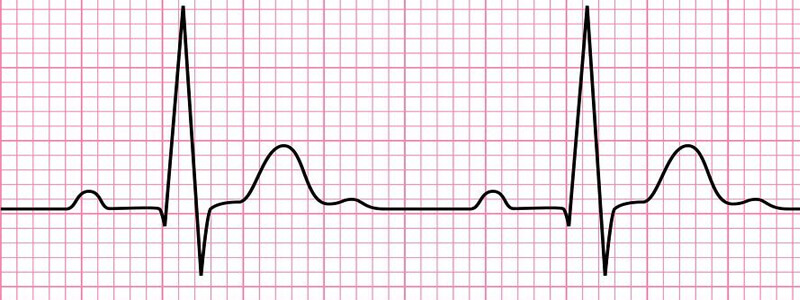
\includegraphics[scale=.]{image/week1/intro.jpg}
     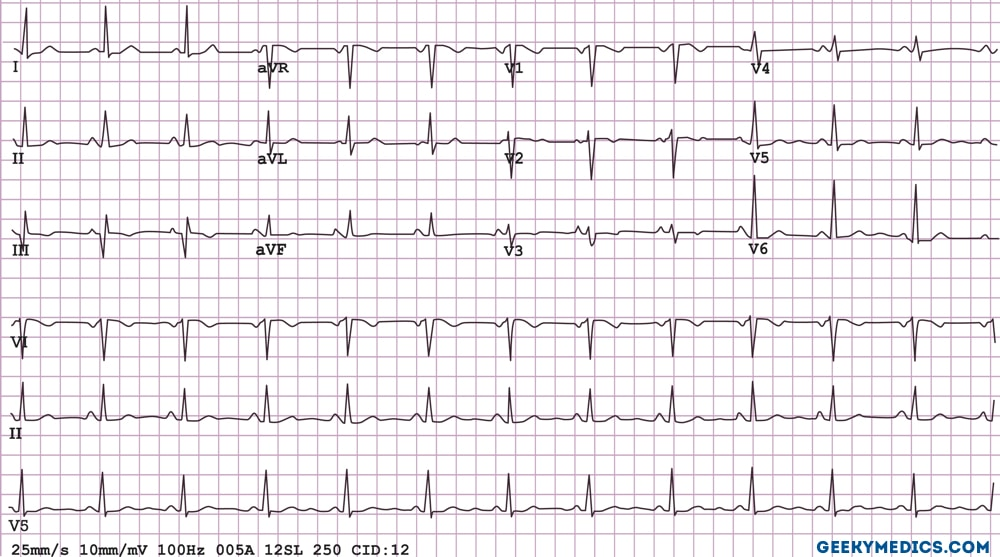
\includegraphics[scale=.35]{image/chapter1/Normal-ECG-SCALED-DOWN-WATERMARK.jpg}
    \end{center}
    \caption{Một đoạn điện tâm đồ }
    \end{figure}
\end{center}

\subsection{Lich sử hình thành điện tâm đồ}
\begin{itemize}
    \item 1887 - Augustus D. Waller (St Mary's Medical School, Luân Đôn) trình bày ECG đầu tiên trên người của Thomas Goswell, một người làm việc trong phòng thử nghiệm.
    \item 1893 - Willem Einthoven giới thiệu từ 'electrocardiogram' tại buổi họp của Hội Y Học Hà Lan (nhưng sau đó ông sửa lại rằng Waller là người đầu tiên dùng chữ này).
    \item 1895 - Einthoven cải tiến dụng cụ và công thức ghi điện, ghi được 5 thay đổi điện trong một nhịp tim, ông ghép chữ cho 5 thay đổi này (P, Q, R, S, T, U).
\end{itemize}

\subsection{Hoạt động điện của cơ tim và sự hình thành điện tâm đồ}
Do sự biến đổi hiệu thế giữa mặt trong và mặt ngoài màng tế bào cơ tim. Sự biến đổi hiệu thế này bắt nguồn từ sự di chuyển của các ion K + , Na + ,... từ ngoài vào trong tế bào và từ trong tế bào ra ngoài khi tế bào cơ tim hoạt động. Lúc này tính thẩm thấu của màng tế bào đối với các ion luôn luôn biến đổi. Do sự chênh lệch nồng độ hai bên màng tạo nên hiệu điện thế giữa hai bên màng (điện thế nghỉ).
\begin{center}
    \begin{figure}[htp]
    \begin{center}
     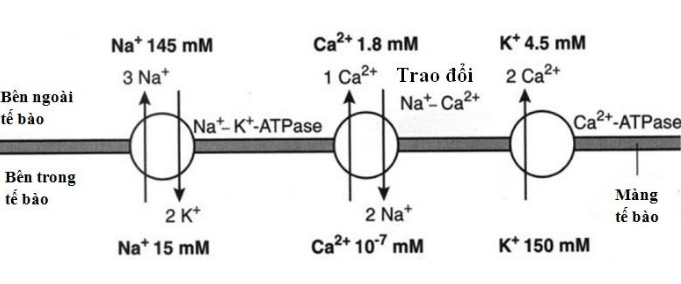
\includegraphics[scale=.4]{image/week1/h21.png}
    \end{center}
    \caption[Sự chênh lệch nồng độ của các ion]{Sự chênh lệch nồng độ của các ion Na, K, Ca trong cơ chế hình thành điện tâm đồ \cite{huongdanDTT}}
    \end{figure}
\end{center}

Tim người có 4 buồng để chứa và bơm máu. Hai phần nhỏ ở phía trên gọi là tâm nhĩ (vì trông giống lỗ tai). Hai phần dưới lớn hơn gọi là tâm thất. Máu theo tĩnh mạch từ cơ thể trở về tâm nhĩ phải, từ phổi trở về tâm nhĩ trái. Tâm nhĩ trái bóp bơm máu vào tâm thất trái, tâm nhĩ phải đưa máu vào tâm thất phải. Sau đó tâm thất phải bóp để bơm máu theo động mạch lên phổi và tâm thất trái bóp để bơm máu xuống cơ thể. Tim có khả năng hoạt động đều đặn và thứ tự như thế là nhờ một hệ thống các tế bào dẫn điện đặc biệt nằm trong cơ tim.

Trong tâm nhĩ bên phải có nút xoang nhĩ (sinoatrial node) gồm các tế bào có khả năng tự tạo xung điện (electric impulse). Xung điện này truyền ra các cơ chung quanh làm co bóp hai tâm nhĩ (tạo nên sóng P trên Điện Tâm đồ). Sau có dòng điện tiếp tục truyền theo 1 chuỗi tế bào đặc biệt tới nút nhĩ thất (atrioventricular node) nằm gần vách liên thất rồi theo chuỗi tế bào sợi Purkinje chạy dọc vách liên thất lan vào các cơ chung quanh (loạt sóng QRS) làm hai thất này co bóp. Sau đó xung điện giảm đi, tâm thất giãn ra (tạo nên sóng T).

\subsection{Các sóng cơ bản và sự hình thành phức bộ sóng}
Một chu kỳ tim biểu hiện trên điện tâm đồ là: sóng P, phức bộ QRS, sóng T, và sóng U (nếu có), hình dạng, thời gian kéo dài của sóng/phức bộ và cả thời gian giữa các thành phần với nhau đều có ý nghĩa đặc biệt quan trọng trong việc chẩn đoán.
\begin{center}
        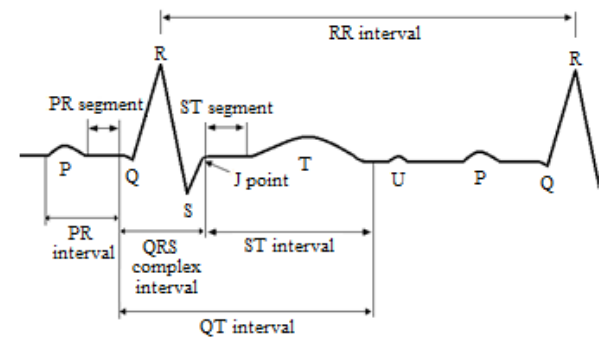
\includegraphics[scale=.4]{image/week1/h32.png}
        \begin{figure}[htp]
        \begin{center}
        \end{center}
        \caption{Tổng hợp những sóng cơ bản}
        \end{figure}
\end{center}

\subsubsection{Các sóng và phức bộ}
\textbf{Sóng P}

Sóng P hình thành do quá trình khử cực tâm nhĩ (cả nhĩ trái và nhĩ phải), bình thường biên độ của sóng P thường dưới 2mm (0.2mmV), và thời gian của sóng P là từ 0.08 đến 0.1 giây, việc tăng biên độ và kéo dài thời gian của sóng gợi ý đến một tình trạng tâm nhĩ lớn (tăng biên độ gợi ý lớn nhĩ phải. thời gian khử cực kéo dài gợi ý đến lớn nhĩ trái).

\textbf{Phức bộ QRS}

Phức bộ QRS thể hiện quá trình khử cực của tâm thất, tùy vào chiều khử cực và vị trí đặt điện cực mà trên giấy ghi sẽ cho thấy các phức bộ khác nhau, ưu thế sóng R hay S, bình thường QRS kéo dài từ 0.06 đến 0.1 giây.
\begin{itemize}
    \item Sóng Q là sóng âm đầu tiên của phức bộ QRS, sóng Q trên bệnh nhân bình thường thường nhỏ và ngắn (hình thành do quá trình khử cực vách liên thất), một sóng Q sâu (biên độ âm lớn) và kéo dài cho thấy một tình trạng hoại tử cơ tim (Trong nhồi máu cơ tim cũ hay nhồi máu cơ tim không có ST chênh lệch).
    \item Sóng R là sóng dương đầu tiên của phức bộ, và sóng âm sau nó là S, đây là hai sóng hình thành do khử cực thất, về bản chất là giống nhau, nếu điện cực đặt ở vị trị chiều khử cực hướng đến thì sóng R sẽ ưu thế, như trong chuyển đạo DII, V5, V6. Sóng R sẽ ưu thế hơn nếu chiều khử cực đi xa vị trí đặt điện cực như V1, V2.
\end{itemize}

\textbf{Sóng T}

Là sóng theo sau phức bộ QRS, thể hiện quá trình tái cực muộn của 2 tâm thất, sóng T có giá trị rất lớn trong việc nhận định một tình trạng cơ tim thiếu máu.
\textbf{Sóng U}
Nguồn gốc sóng U vẫn chưa điện xác định rõ ràng, các giả thuyết đặt ra là:
\begin{itemize}
    \item Tái cực chậm sợi Purkinje.
    \item Tái cực kéo dài giữa cơ tim tế bào M (mid-myocardial cell).
    \item Sau kết quả điện thế của trương lực cơ trong các thành tâm thất.
\end{itemize}
Bình thường không thấy sóng U trên điện tâm đồ, nếu có thì là sóng nhỏ sau sóng T, sóng U đảo ngược hay nhô cao nhọn gặp trong rất nhiều loại bệnh lý tim (bệnh mạch vành, tăng huyết áp, bệnh van tim, tim bẩm sinh, bệnh lý cơ tim, cường giáp, ngộ độc, rối loạn điện giải,...)
\subsubsection{Các đoạn - khoảng}
\textbf{Khoảng PQ}

Là thời gian dẫn truyền từ nhĩ đến thất, bình thường từ 0.12 - 0.2 giây, việc kéo dài thể hiện quá trình chậm dẫn truyền (do bị block), PQ ngắn sẽ gợi ý đến một hội chứng kích thích sớm (Wolf-Parkinson-White)

\textbf{Đoạn ST}

Ý nghĩa là giai đoạn tái cực thất sớm, thời gian của ST thường không quan trọng bằng hình dạng của nó, bình thường ST nằm chênh lệch lên hoặc chênh xuống khỏi đường đẳng điện rất ít. đoạn ST cực kỳ quan trọng trong việc chẩn đoán nhồi máu cơ tim.

ST gọi là chênh lệch nếu cao hơn đường đẳng điện 1mm ở chuyển đạo chi và hơn 2mm ở chuyển đạo trước ngực

ST gọi là chênh xuống khi nằm dưới đường đẳng điện hơn 0.5mm

\textbf{Đoạn QT}

Là thời gian tâm thu điện học của tâm thất, khoảng giá trị bình thường của QT phục thuộc vào tần số tim, QT kéo dài bất thường có liên quan với tăng nguy cơ loạn nhịp thất, đặc biệt là xoắn đỉnh. Gần đây, hội chứng QT ngắn bẩm sinh đã được tìm thấy có liên quan với tăng nguy cơ rung nhĩ và thất kịch phát và đột tử do tim.

\subsection{Các chuyển đạo thông dụng}

\subsubsection{Điện trường tim}
Cơ thể con người là một môi trường dẫn điện; vì thế, dòng điện do tim phát ra được dẫn truyền khắp cơ thể, ra tới da, biến cơ thể thành một điện trường của tim. Nếu ta đặt hai điện cực lên bất cứ hai điểm nào đó có điện thế khác nhau của điện trường đó, ta sẽ thu được một dòng điện thể hiện hiệu thế giữa hai điểm đó và gọi là một chuyển đạo hay đạo trình (lead). Nó hiện ra trên máy ghi bằng một đường cong điện tâm đồ có một hình dạng nào đó tùy theo địa điểm đặt các điện cực. Đường thẳng nối hai địa điểm đặt điện cực trên cơ thể gọi là trục chuyển đạo.

\subsubsection{Chuyển đạo mẩu:}
\begin{center}
    \begin{figure}[htp]
    \begin{center}
    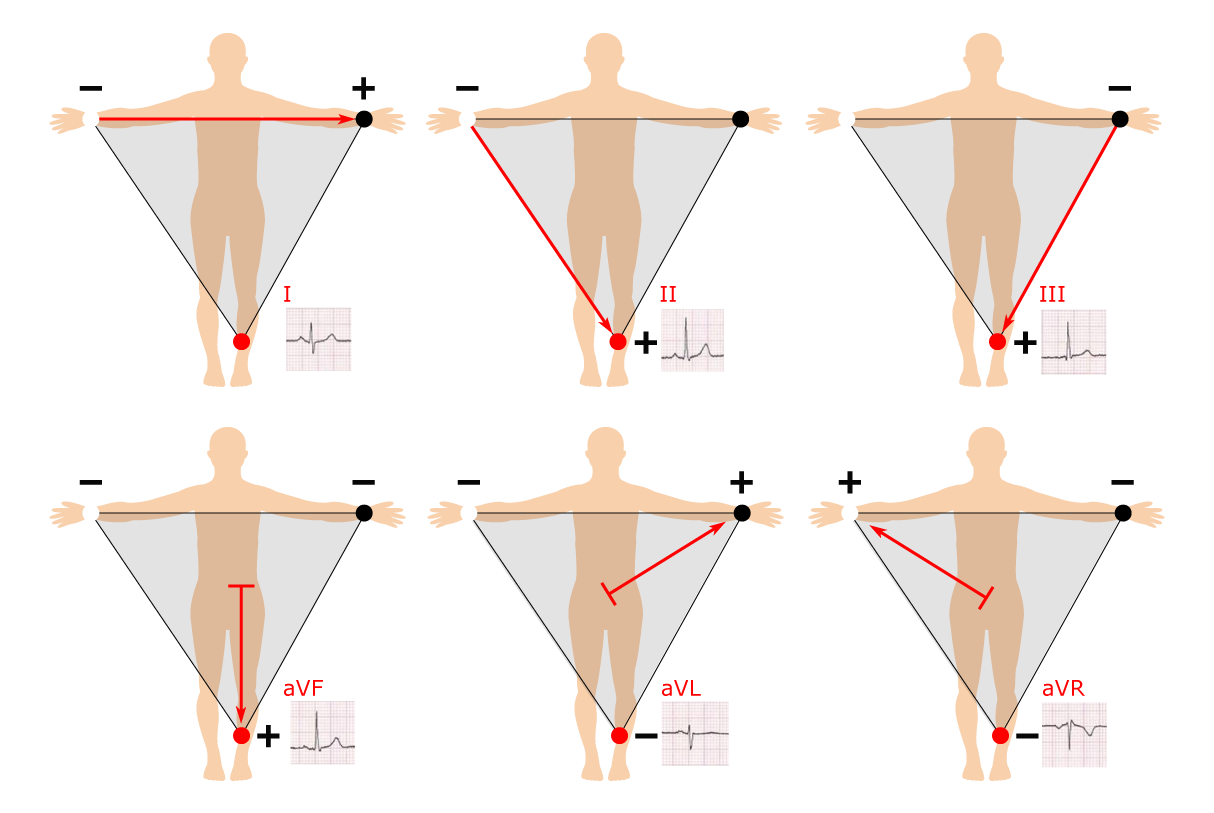
\includegraphics[scale=.2]{image/week1/chuyendaochi.png}
    \end{center}
    \caption[Chuyển đạo chi]{Chuyển đạo chi \cite{chuyendao}}
    \end{figure}
\end{center}
Tất cả 6 chuyển đạo: D1, D2, D3, aVR, aVL, aVF được gọi chung là các chuyển đạo ngoại biên vì đều có điện cực thăm dò đặt ở các chi. Chúng hỗ trợ cho nhau “dò xét” các rối loạn của dòng điện tim thể hiện ở bốn phía xung quanh quả tim trên mặt phẳng chắn (frontal plane).
\begin{center}
    \begin{figure}[htp]
    \begin{center}
    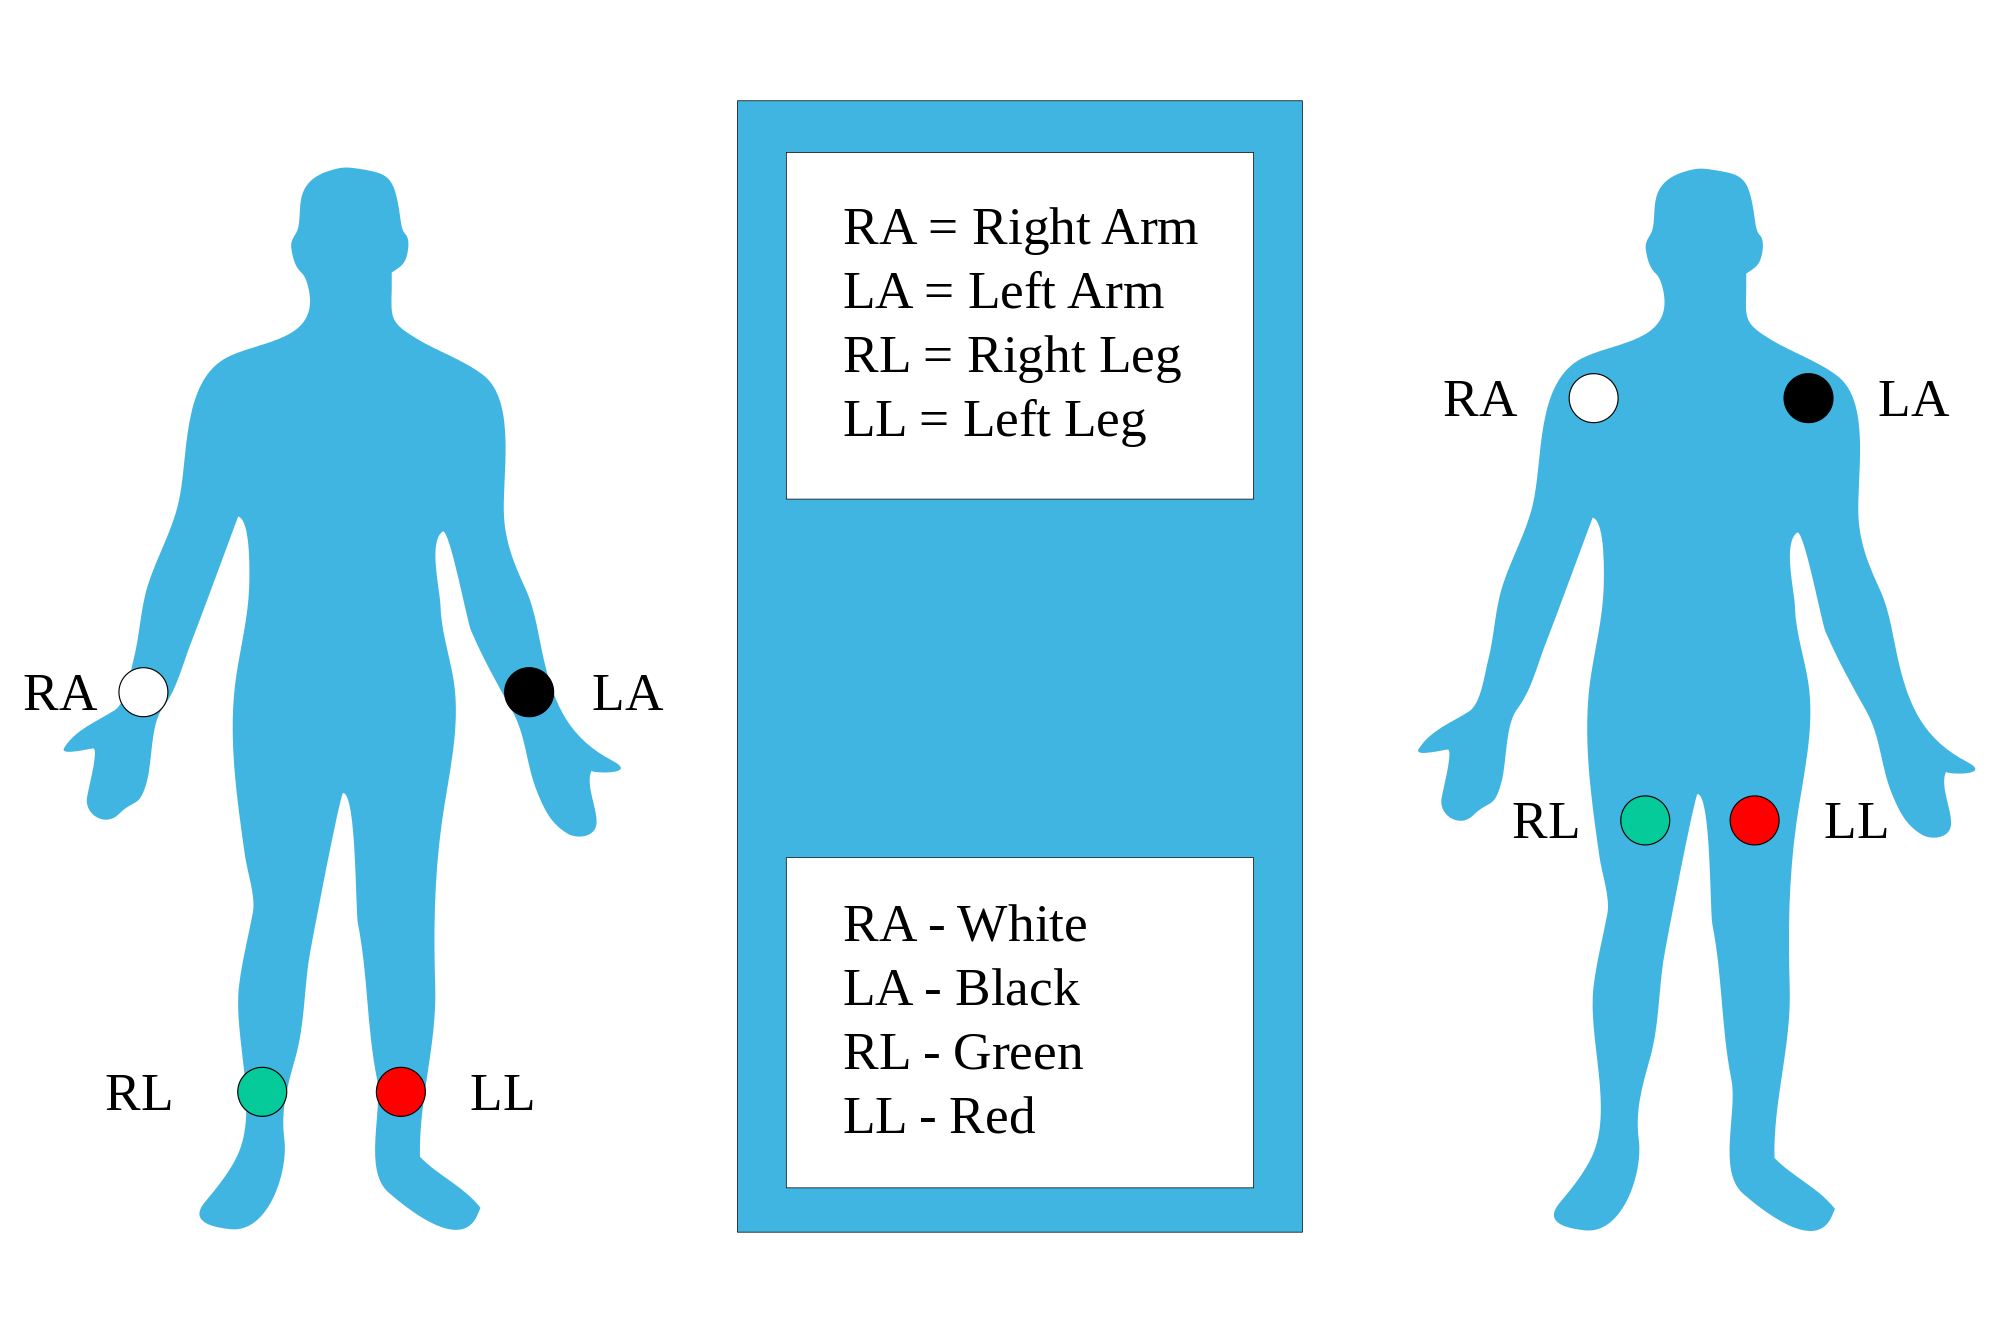
\includegraphics[scale=.12]{image/chapter1/2000px-Limb_leads.png}
    \end{center}
    \caption{Các vị trí đặt điện cực}
    \end{figure}
\end{center}

\subsubsection{Chuyển đạo trước tim:}
\begin{center}
    \begin{figure}[htp]
    \begin{center}
    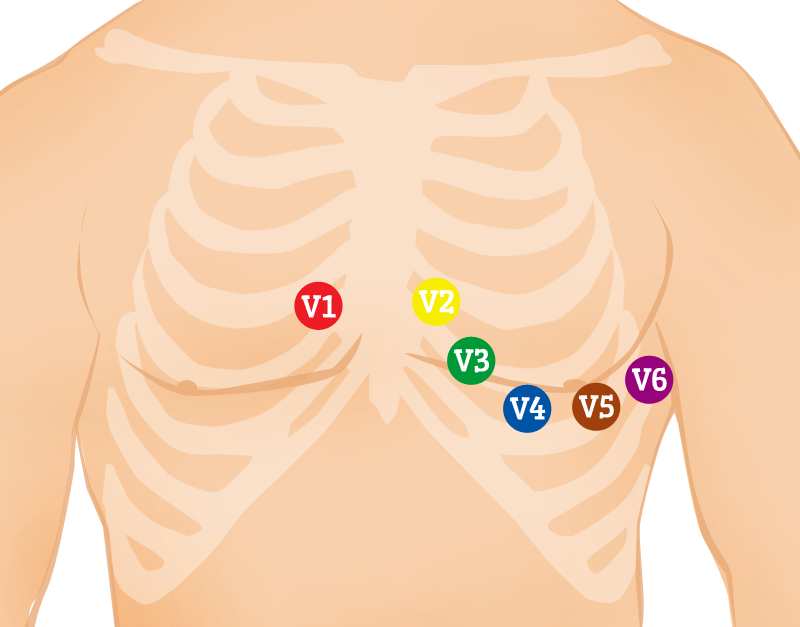
\includegraphics[scale=.25]{image/week1/chuyendaotruocnguc.png}
    \end{center}
    \caption{Chuyển đạo trước tim}
    \end{figure}
\end{center}
Người ta thường ghi đồng loạt cho bệnh nhân 6 chuyển đạo trước tim thông dụng nhất, kí hiệu bằng chữ V (voltage) kèm theo các chỉ số từ 1 đến 6.(V1, V2,…,V6).

\subsubsection{Một số chuyển đạo khác:}
V7, V8, V9(điện cực ở mé trái và sau lồng ngực dùng để thăm dò thất trái), V3R, V4R, V5R, V6R(điện cực ở mé phải lồng ngực dùng để nghiên cứu thất phải hay tim sang phải), chuyển đạo thực quản (Kí hiệu VOE), chuyển đạo trong buồng tim, điện đồ His.

\subsection{Đo điện tâm đồ}
\subsubsection{Đo điện tâm đồ truyền thống}
Định dạng chuẩn của một điện tâm đồ là điện tâm đồ được ghi lại trên một khổ giấy
.Để đánh giá thời gian dài hay ngắn và biên độ cao hay thấp của các làn sóng điện tâm đồ, người ta đinh chuẩn: 
\begin{itemize}
    \item Vận tốc 25mm/s thì mỗi ô 1mm có giá trị 0,04s.
    \item Theo chiều ngang 1 ô lớn tương ứng với 1000ms.
    \item Theo chiều dọc 1 ô lớn tương ứng 500mV.
\end{itemize}
\begin{center}
    \begin{figure}[htp]
    \begin{center}
    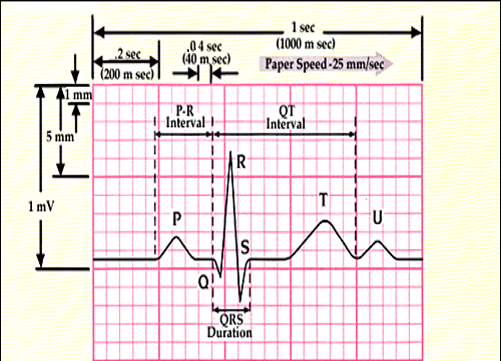
\includegraphics[scale=.6]{image/week1/new_ecg_paper.png}
    \end{center}
    \caption[Hình ảnh một chu kỳ sóng]{Hình ảnh một chu kỳ sóng được đo theo kích thước khổ giấy, bác sĩ căn cứ vào ô trên giấy để phát hiện bất thường ở ECG \cite{ecggiay}}
    \end{figure}
\end{center}
\subsubsection{Đo điện tâm đồ bằng thiết bị di động thông minh (Apple Watch Series 4)}
Tính năng ECG hay còn gọi là đo điện tâm đồ đã chính thức có thể sử dụng trên Apple Watch Series 4 để phát hiện nhịp tim bất thường và chẩn đoán các bệnh tim nghiêm trọng.
\begin{center}
    \begin{figure}[htp]
    \begin{center}
    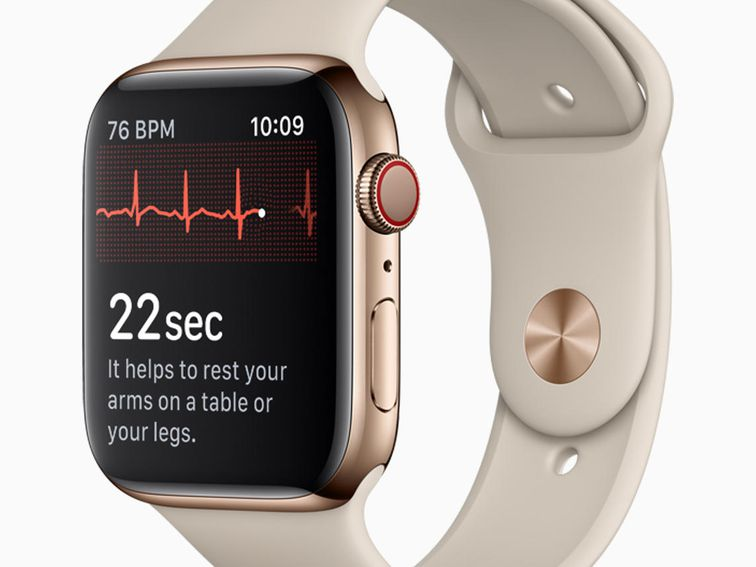
\includegraphics[scale=.3]{image/chapter1/apple-watch-series4-ecg-crown-09122018.jpg}
    \end{center}
    \caption{Apple Watch Series 4}
    \end{figure}
\end{center}
% \section{Đọc một điện tâm đồ}
% \subsection{Những bước phân tích trước khi đọc một điện tâm đồ}
% Điện tâm đồ (ECG) là một đường cong ghi lại các biến thiên của các điện lực do tim phát ra trong khi hoạt động co bóp.\cite{huongdanDTT}

% \begin{enumerate}
%     \item Trước khi đọc điện tâm đồ, phải nắm vững tuổi, giới tính, chẩn đoán lâm sàng của bệnh
%     nhân. Ngoài ra, còn nên biết thêm sơ lược bệnh án, hình ảnh X quang, các kết quả xét nghiệm khác và nhất là hai vấn đề sau đây:
%     \begin{itemize}
%         \item Khổ người bệnh nhân gầy béo, cao thấp ảnh hưởng rất nhiều đến tư thế tìm và biên độ sóng, nó ảnh hưởng nhiều đến chẩn đoán dày thất.
%         \item Có đang dùng thuốc trợ tim hay thuốc chống loạn nhịp dài ngày không? Nhất là digitan và quinidin… vì các thuốc này tác động rất nhiều đến hình dạng điện tâm đồ và dễ làm sai lạc chẩn đoán cơ bản.
%     \end{itemize}
%     \item Kiểm tra kỹ thuật ghi điện tâm đồ, phát hiện ghi sai, ảnh hưởng tạp, milivôn lấy đúng 1cm
%     hay không? Tốc độ ghi bao nhiêu? Nghĩa là các đường kẻ dọc cách nhau bao nhiêu phần trăm
%     giây
%     \item Nhịp tim: bước vào đọc điện tâm đồ trước hết bao giờ cũng phải xem nhịp xoang hay
%     không xoang? Có những rối loạn nhịp tim gì? Đừng bao giờ quên tính tần số tim. Nếu có blốc
%     nhĩ-thất thì phải tính riêng cả tần số nhĩ.
%     \item Trục điện tim với góc alpha, tư thế tim.
%     \item Hình dạng các sóng: đọc đồng thời ở cả 12 chuyển đạo thông dụng:
%     \begin{itemize}
%         \item Sóng P: chiều cao (biên độ), chiều rộng (thời gian), hình dạng (âm, dương, hai pha, móc).
%         \item Khoảng PQ dài bao nhiêu?
%         \item Phức bộ QRS: biên độ và thời gian chung và riêng của sóng Q, hình dạng (móc…).
%         \item Riêng với V1 và V5 thì tìm thêm thời gian xuất hiện nhánh nội điện.
%         \item Đoạn ST có chênh không?
%         \item Sóng T (và sóng U): dạng (dương, âm hay hai pha), biên độ.
%         \item Khoảng QT dài bao nhiêu?
%     \end{itemize}
%     \item Kết luận chẩn đoán: về tổn thương cơ tim và về rối loạn nhịp tim.
% \end{enumerate}


\section{Tìm hiểu một số nghiên cứu liên quan}
\thispagestyle{fancy}
\textbf{Trong nghiên cứu của KS Park và các cộng sự đã sử dụng kỹ thuật SVM phân lớp (Hierarchical Support Vector Machine)} áp dụng phương pháp thống kê đề xuất bậc cao (higher order statistics-HOS) và hàm căn bản Hermite(HBF) để phân loại các nhóm bệnh tim. Theo như nghiên cứu, phức bộ QRS của ECG đóng vai trò rất quan trọng trong nghiên cứu tuy nhiên đặc điểm về hình thái của phức bộ QRS trong lớp N và lớp S khá giống nhau, lớp F và V cũng vậy (các lớp này là label cho việc phân loại, cũng là ký hiệu cho các loại bệnh). Vì vậy, nhóm nghiên cứu đã cân nhắc sử dụng mô hình phân lớp sử dụng SVM để phân loại các lớp có hình thù sóng giống nhau đó. Quá trình phân loại có 2 phase. Ở phase đầu, tiến hành phân loại dữ liệu thành 2 nhóm: nhóm NS và nhóm FV sử dụng HOS,  HBF và những khoảng đặc trưng QRS. Ở phase thứ 2, để phân loại N và S nhóm chỉ sử dụng khoảng RR của dữ liệu. Đối với phân loại V và F ở phase 2, nhóm đã sử dụng toàn bộ đặc trưng đã trích xuất được để thực hiện (bao gồm: khoảng QRS, khoảng RR, trung bình độ dài RR, tỉ số của độ dài RR và trung bình RR). Kết quả cho thấy hệ thống phân loại khá tốt các loại bệnh trong điều kiện phân phối dữ liệu không cân bằng điều mà những hệ thống thông thường chưa đạt được.

\textbf{Trong nghiên cứu của Ozcan và Gurgen đã kết hợp SVM với hướng tiếp cận mờ (fuzzy)} gọi tắt là fuzzy-SVM (FSVM). Phương pháp FSVM định nghĩa mờ input và gán những giá trị thành viên (membership value) cho mỗi input. Ý tưởng của nghiên cứu rất đơn giản đó là sử dụng những cách tiếp cận mờ để định nghĩa trọng số cho input sau đó dùng SVM để phân loại chúng dựa trên những trọng số đã định nghĩa. FSVM giới thiệu khái niệm giá trị thành viên vào SVM dẫn đến việc định nghĩa những hàm thành viên. Một giá trị thành viên cung cấp một bậc (degree) của việc đại diện input cho lớp đó vì vậy một số hàm thành viên được đề xuất trong nghiên cứu: OCW, DTCM, DTOCM, CAR, FCM. Qua nhiều thử nghiệm của nhóm nghiên cứu thì phương pháp FSVM-DTCM đem lại độ chính xác (accuracy) tốt nhất được kiểm nghiệm bằng kỹ thuật 10 fold cross-validation.

\textbf{Andrew Ng và nhóm nghiên cứu đã đề xuất mô hình Convolutional neural network} gồm 34 layers để phân loại chuỗi tín hiệu ECG. Mô hình có thể dự đoán chính xác giữa nhịp xoang (SINUS) và rung nhĩ (AFIB) điều mà nhiều giải thuật khác không làm được. Trước khi cho vào mạng phân loại, dữ liệu sẽ đươc chuẩn hóa để resample. Trước mỗi convolution layer nhóm áp dụng Batch Normalization và một rectified linear activation. Nhóm cũng áp dụng kỹ thuật Dropout giữa các convolution layer và sau các hàm phi tuyến. Cuối cùng là lớp fully connected với hàm kích hoạt softmax gồm 14 lớp output.

\textbf{Saxena và cộng sự trong \cite{classify} đã mô tả một cách tiếp cận đối với các tín hiệu ECG dạng trích xuất tính năng hiệu quả}. Bài báo của họ đề cập đến một phương pháp tổng hợp được phát triển để nén dữ liệu, truy xuất tín hiệu và trích xuất đặc trưng của tín hiệu ECG. Sau khi lấy tín hiệu từ dữ liệu nén, người ta thấy rằng mạng không chỉ nén dữ liệu mà còn cải thiện chất lượng tín hiệu ECG được truy xuất liên quan đến việc loại bỏ nhiễu tần số cao có trong tín hiệu gốc. Với việc triển khai mạng nơ ron nhân tạo (ANN), tỷ lệ nén tăng khi số chu kỳ ECG tăng. Ngoài ra, các tính năng được trích xuất theo tiêu chí biên độ, độ dốc và thời lượng từ tín hiệu thu được khớp với các tính năng của tín hiệu gốc. Kết quả thử nghiệm của họ ở mọi giai đoạn đều đều và ổn định và chứng minh rằng không thể nghi ngờ rằng phương pháp tổng hợp có thể được sử dụng để quản lý dữ liệu hiệu quả và trích xuất tính năng của tín hiệu ECG trong nhiều ứng dụng thời gian thực.

\textbf{Pyakillya và các công sự \cite{cnn1d} Đã tiếp cận theo hướng sử dụng Convolution layer 1D kết hợp với Fully Connected layer} trong phân loại nhịp tim (nhịp xoang bình thường, rối loạn nhịp, các loại nhịp khác và nhiễu loạn). Cụ thể, trong mô hình do Pyakillya đề xuất phần trích xuất đặc trưng áp dụng CNN một cách đặc biệt. Chi tiết kiến trúc mô hình phần loại gồm: 7 convolutional layers với số bộ lọc ngang là 5 and 128 neurons + max-pooling áp dụng dropout cho mỗi layer + GlovalAveragePooling + 3 FCN layers with (256/128/64) neurons + dropout sau mỗi layers + softmax layer cho 4 outputs. Kết quả phân loại thu được cho thấy giải pháp của nhóm nghiên cứu đề xuất có thể phân loại tốt các loại nhịp của ECG trong điều kiện dữ liệu không có cấu trúc rõ ràng và không cân bằng. Ngoài ra giải pháp đề xuất có thể tự trích xuất những thông tin đặc trưng của dữ liệu mà không cần bất kì chuyên gia y tế hay chuyên gia liên quan nào. Tuy nhiên về độ hiệu quả và độ chính xác của giải pháp chưa được cao như những nghiên cứu khác liên quan.


% \section{Tiền xử lý tín hiệu}
% Điện tâm đồ (ECG) là một trong những tín hiệu điện sinh học và nó được sử dụng để ghi lại các hoạt động điện của tim. Tín hiệu của ECG được đặc trưng bởi các sóng PQRS. Loại tín hiệu điện sinh học này chủ yếu được sử dụng trong lâm sàng để xác định các bệnh tim ở Bệnh nhân. Các điện cực bề mặt được sử dụng để đo tín hiệu ECG. Một số nhiễu loạn được tạo ra thông qua điện cực bề mặt này, có thể do các điện cực không được đặt đúng cách trong bệnh nhân. Một số bước để loại bỏ nhiễu về cơ bản là:
% \begin{itemize}
%     \item Kiểm tra da bệnh nhân, tiến hành và chuẩn bị da tốt cho bệnh nhân.
%     \item Kiểm tra gel điện cực.
%     \item Trong thời gian kiểm tra bệnh nhân nên
%     được giữ ấm, không nói và di chuyển.
%     \item Kiểm tra chuyển đạo trước ngực được đặt đúng vị trí hay không. Nếu nó không được đặt đúng cách có nghĩa là nó dẫn đến chẩn đoán sai về
%     nhồi máu cơ tim.
%     \item Kiểm tra kết nối cáp Bệnh nhân với thiết bị ECG
% \end{itemize}
% Đây là những cách được xử lý để loại bỏ nhiểu trong lúc đo tại các trung tâm y tế khi đo điện tâm đồ . Tuy nhiên vẫn còn tồn đọng rất nhiều nhiễu loại như: lệch đường đẳng điện, nhiễu do chuyển động, nhiễu do tiếp xúc các điện cực, nhiễu của thiết bị đo,...Những loại nhiễu loạn này được xử lý bằng nhiều kỹ thuật xử lý tín hiệu. Một số bộ lọc được Rajkumar Patro và nhóm nghiên cứu sử dụng để lọc nhiễu như: Median Filter, Gaussian Filter, Low-pass Butterworth Filter, Window based FIR Filter được thực hiện trên bộ dữ liệu MIT-BIH và đánh giá bằng các độ đo số toàn phương trung bình (MSE) và PSNR. Bên cạnh đó một số kỹ thuật gần đây cũng được áp dụng để lọc nhiễu như: Principle Component Analysis, Neural Network và Wavelet transform, đặc biệt chỉ loại được những tần số cao khỏi sóng và có nhược điểm là băng thông của nó không phải hằng số \cite{130540},\cite{948947}. Karol Antczak đề xuất sử dụng Mạng hồi quy sâu để lọc nhiễu (Deep Recurrent Neural Network) cũng giải quyết được những vấn để trên.

% \section{Trích xuất đặc trưng tín hiệu điện tâm đồ }
% \subsection{Trích xuất đặc trưng}
% Trích xuất đặc trưng tín hiệu điện tim đóng vai trò quan trọng trong chuẩn đoán bệnh tim. Một chu kỳ của nhịp tim gồm các thành phần sóng cơ bản P,Q,R,S,T. Biên độ và chiều dài các thành phần sóng xác định chức năng tim của mỗi con người.\par
% Zhao và cộng sự. [6] đề xuất một phương pháp trích xuất tính năng bằng cách sử dụng wavelet transform và support vector machine. Bài viết trình bày một cách tiếp cận mới để trích xuất đặc trưng để nhận biết nhịp tim đáng tin cậy. Hệ thống phân loại được đề xuất bao gồm ba thành phần bao gồm tiền xử lý dữ liệu, trích xuất đặc trưng và phân loại tín hiệu ECG. Hai phương pháp trích xuất tính năng đa dạng được áp dụng cùng nhau để đạt được vector đặc trưng của dữ liệu ECG. Biến đổi wavelet được sử dụng để trích xuất các hệ số của biến đổi như các tính năng của từng phân đoạn ECG. Đồng thời, mô hình tự phát (AR) cũng được áp dụng để nắm giữ các cấu trúc thời gian của dạng sóng ECG. Sau đó, cuối cùng, support vector machine (SVM) với Gaussian kernel được sử dụng để phân loại nhịp tim ECG khác nhau. Kết quả mô phỏng máy tính được cung cấp để xác định hiệu suất của phương pháp đề xuất đạt độ chính xác tổng thể là 99,68\%.\par
% Một cách tiếp cận mới để trích xuất đặc trưng ECG đã được đưa ra bởi Fidel và các cộng sự trong [7]. Bài báo đề xuất của họ trình bày một thuật toán, dựa trên biến đổi wavelet, để trích xuất tính năng từ tín hiệu điện tâm đồ (ECG) và nhận biết nhịp tim bất thường. Vì các phép biến đổi wavelet có thể được định vị cả trong miền tần số và thời gian. Họ đã phát triển một phương pháp để chọn một sóng mẹ tối ưu từ một tập hợp ngân hàng bộ lọc sóng con trực giao và trực giao bằng phương pháp tương quan tốt nhất với tín hiệu ECG. Bước đầu tiên trong cách tiếp cận của họ là khử nhiễu (loại bỏ nhiễu) tín hiệu ECG bằng ngưỡng mềm hoặc cứng với giới hạn 99,99 tái tạo khả năng và sau đó mỗi chu kỳ PQRST được phân tách thành một vectơ hệ số bằng hàm sóng con tối ưu. Các hệ số, xấp xỉ của mức tỷ lệ cuối cùng và chi tiết của tất cả các cấp, được sử dụng cho ECG được phân tích. Họ đã chia các hệ số của mỗi chu kỳ thành ba phân đoạn có liên quan đến sóng P, phức bộ QRS và sóng T. Tổng các giá trị từ các phân đoạn này đã cung cấp các vectơ đặc trưng của các chu kỳ đơn.\par
% Mahmoodabadi và cộng sự. trong [1] đã mô tả một cách tiếp cận để trích xuất tính năng ECG sử dụng phép biến đổi Daubechies Wavelets. Họ đã phát triển và đánh giá một hệ thống trích xuất điện tâm đồ (ECG) dựa trên biến đổi sóng con đa độ phân giải. Các tín hiệu ECG từ Modified Lead II (MLII) đã được chọn để xử lý. Bộ lọc wavelet với chức năng chia tỷ lệ gần giống với hình dạng của tín hiệu ECG đạt được phát hiện tốt hơn. Bước đầu tiên trong phương pháp của họ là khử nhiễu tín hiệu ECG bằng cách loại bỏ các hệ số sóng con tương đương ở quy mô cao hơn. Sau đó, các phức bộ QRS được phát hiện và mỗi một phức được sử dụng để theo dõi các đỉnh của các sóng riêng lẻ, bao gồm các bộ và sóng của sóng P và T có trong một chu kỳ tim. Kết quả thử nghiệm của họ cho thấy phương pháp tiếp cận được đề xuất của họ cho trích xuất tính năng ECG đạt được độ nhạy (sensitivity) 99,18\% và dự đoán tích cực (positive predictivity) là 98\%.\par
% Saxena và cộng sự trong [10] đã mô tả một cách tiếp cận đối với các tín hiệu ECG dạng trích xuất tính năng hiệu quả. Bài báo của họ đề cập đến một phương pháp tổng hợp được phát triển để nén dữ liệu, truy xuất tín hiệu và trích xuất đặc trưng của tín hiệu ECG. Sau khi lấy tín hiệu từ dữ liệu nén, người ta thấy rằng mạng không chỉ nén dữ liệu mà còn cải thiện chất lượng tín hiệu ECG được truy xuất liên quan đến việc loại bỏ nhiễu tần số cao có trong tín hiệu gốc. Với việc triển khai mạng nơ ron nhân tạo (ANN), tỷ lệ nén tăng khi số chu kỳ ECG tăng. Ngoài ra, các tính năng được trích xuất theo tiêu chí biên độ, độ dốc và thời lượng từ tín hiệu thu được khớp với các tính năng của tín hiệu gốc. Kết quả thử nghiệm của họ ở mọi giai đoạn đều đều và ổn định và chứng minh rằng không thể nghi ngờ rằng phương pháp tổng hợp có thể được sử dụng để quản lý dữ liệu hiệu quả và trích xuất tính năng của tín hiệu ECG trong nhiều ứng dụng thời gian thực.\par
% Một trong những tính chất chung của ECG là đoạn trong R-R (R-R interval) hay nói cách khác là khoản cách từ đỉnh R của chu kỳ sóng này đến đỉnh R của chu kỳ sóng kia. Ngoại trừ những bệnh nhân sử dụng máy tạo nhịp tim, những thay đổi về độ rộng của đoạn R-R có liên quan đến hình thái đường cong của nhịp tim, và những biến đổi này thường là dấu hiệu của việc rối loạn nhịp tim. Vì vậy, các đặc trưng trong khoảng RR có khả năng lớn để phân biệt các loại nhịp tim và một số tác giả áp dụng các phương pháp của mình chỉ dựa vào các đặc trưng khoảng RR [67-69].\par
% Lin và Yang [41] đã chỉ ra rằng việc sử dụng khoảng R-R chuẩn hóa giúp cải thiện đáng kể kết quả phân loại. Chỉ các khoảng RR chuẩn hóa được sử dụng trong nghiên cứu đó và kết quả có thể so sánh với các phương pháp tiên tiến ngay cả trong mô hình liên bệnh nhân. Doquire và các đồng nghiệp [71] đã xác nhận hiệu quả của các khoảng RR được chuẩn hóa bằng các kỹ thuật lựa chọn đặc trưng.\par
% Các đặc trưng từ miền thời gian/tần số của các đặc trưng trong khoảng R-R được sử dụng trong các nghiên cứu gần đây đem lại sự chính xác cao nhất cho mô hình phân loại. Nhằm mục đích giảm kích thước của vectơ đặc trưng,...các kỹ thuật khác nhau đã được áp dụng trực tiếp trên các mẫu (samples) đại diện cho nhịp tim (trong vùng lân cận của đỉnh R) như phân tích thành phần chính (PCA) [75-77] hoặc phân tích thành phần độc lập ( ICA) [78-80], trong đó các hệ số mới được trích xuất để biểu thị nhịp tim. Chawla [81] trình bày một nghiên cứu so sánh giữa việc sử dụng PCA và ICA để giảm nhiễu và tạo tín hiệu của tín hiệu ECG và cho thấy PCA là một kỹ thuật tốt hơn để giảm nhiễu, trong khi ICA là phương pháp tốt hơn để trích xuất các tính năng. Kỹ thuật ICA cho phép tách riêng các nguồn riêng biệt khỏi tín hiệu trộn. Hơn nữa, người ta đã chứng minh rằng sự kết hợp của hai kỹ thuật này, tức là PCA để giảm nhiễu và ICA để trích xuất tính năng, có thể mang lại lợi thế lớn hơn khi so sánh chỉ sử dụng một trong số chúng.

% \section{Phân loại điện tim}
% Khi tập hợp các đặc trưng đã được xác định từ nhịp tim, ta có thể áp dụng mô hình phân loại bằng những kĩ thuật học máy, học sâu. Có 4 kỹ thuật phổ biến được sử dụng trong các nghiên cứu về phân loại điện tim từ trước đến nay.\par
% Support Vector Machine (SVM) là một trong những phân loại phổ biến nhất được tìm thấy trong tài liệu cho các phương pháp phân loại rối loạn nhịp tim dựa trên ECG. Park và cộng sự [7] đã sử dụng SVM trong cấu hình phân cấp giả để giải quyết sự mất cân bằng của cơ sở dữ liệu MIT-BIH và báo cáo các giá trị đầy hứa hẹn. de Lannoy và cộng sự [32] đã cố gắng khắc phục sự mất cân bằng của cơ sở dữ liệu MIT-BIH với SVM. Các cách tiếp cận khác nhau với các biến thể SVM đã được đề xuất, chẳng hạn như kết hợp lý thuyết mờ để tinh chỉnh phân loại SVM [117], kết hợp với một nhóm các phân loại [42], thuật toán di truyền kết hợp với SVM mờ hạn chế [118] và SVM bình phương nhỏ nhất [104]. Huang et al đã sử dụng SVM theo cách phân cấp với chiến lược bỏ phiếu tối đa và báo cáo những cải tiến đáng kể. Moavenian và Khorrami [119] đã đề xuất sử dụng hàm kernel mới để thu thập dữ liệu từ SVM và đã được sử dụng cùng một phương pháp để so sánh các kết quả thu được từ một mạng lưới thần kinh nhân tạo đa lớp (MLP-ANN). Mặc dù SVM hiệu quả hơn trong thời gian thực hiện, cả trong huấn luyện và kiểm thử , MLP hoạt động tốt hơn về accuracy, sensitivity, positive prediction (+ P) và false positive rate (FPR). Vì SVM không hoạt động tốt đối với sự mất cân bằng trong các lớp dữ liệu huấn luyện, các kỹ thuật cân bằng cơ sở dữ liệu cho giai đoạn huấn luyện, ít được khám phá cho vấn đề này, có thể được nghiên cứu trong nghiên cứu trong tương lai để cải thiện SVM.\par
% Kiến trúc mạng neural nhân tạo (ANN) được sử dụng nhiều trong phân loại loạn nhịp là Multilayer Perceptrons (MLP) and Probabilistic Neural Networks (PNN). Theo Yu và Chen [101], các mô hình được xây dựng bằng PNN có tính toán mạnh mẽ và hiệu quả hơn so với MLP truyền thống. Nhiều cách tiếp cận dựa trên ANN cũng được đề xuất. Mar và cộng sự [34] đã so sánh MLP với Phân biệt tuyến tính (Linear Discriminant) và thấy rằng MLP vượt trội hơn đáng kể. Theo Osowski và các đồng nghiệp, việc kết hợp các mô hình phân loại không những giảm thiểu lỗi của mạng neural mà còn giảm tỉ lệ false negatives (NP).\par
% Những kỹ thuật học không giám sát như KNN cũng được đề xuất, tuy nhiên không được sử dụng nhiều trong phân loại điện tim, vì hiệu quả của chúng được liên kết mật thiết với kiến thức trước đó dẫn đến chi phí tính toán cao trong giai đoạn thử nghiệm. Mishra và Raghav [95] đã sử dụng một bộ phân loại dựa trên kNN và báo cáo kết quả đầy hứa hẹn, tuy nhiên chi phí tính toán không được đề cập.\par
% Hidden markov model (HMM) được sử dụng nhiều trong tính hiệu âm thanh và văn bản để phân tích và nhận diện. Coast và các cộng sự [132] dùng HMM cho việc  phân tích và phân loại điện tim.\par
% Phương pháp sử dụng cây quyết định cũng là một trong những phương pháp được đề xuất trong lĩnh vực này. Tuy nhiên, phương pháp này không hiệu quả cho tập dữ liệu số thực liên tục và vector đặc trưng có số chiều lớn. Vì vậy Mert và các cộng sự [147] kết hợp kỹ thuật Bagging và Cây quyết định tạm gọi là Bagged Decision Tree đã đem lại kết quả khá khả quan.\par
% Một số nghiên cứu khác: Trong nghiên cứu \cite{11}, phân loại điện tim dựa trên Neural Network và Fuzzy. Trong nghiên cứu \cite{12}, sự khác nhau giữa sóng bình thường được phân loại bằng cách sử dụng (Linear Discriminant Analysis) LDA and Artificial Neural Networks (ANN). Một số nghiên cứu cho thấy MLP (Multilayer Perception) được dùng trong ANN tốt hơn phân loại LDA. MLP trong ANN được sử dụng để tìm bình thường và bất thường ở ở nhịp tim. Principal component analysis (PCA) và một số cấu trúc neural network được sử dụng và phân loại điện tim. Kết quả của việc này là để tìm ra mô hình neural network phù hợp nhất cho từng loại loạn nhịp khác nhau. Trong nghiên cứu \cite{13}, để thu giảm chiều dữ liệu bằng PCA. Bài báo này đã kết hợp các giải thuật phân cụm giữa FCA và PCA neural networ, và đã chứng minh sự kết hợp này tốt hơn là sử dụng riêng lẻ. Sự so sánh giữa các giải thuật xác định loạn nhịp tim được sử dụng trong nghiên cứu \cite{14}. Trong đó KNN cũng được sử dụng để xác định QRS. Trong nghiên cứu \cite{rnn}, Shraddha Singh và nhóm nghiên cứu đã phân loại ECG bằng mạng Neuron hồi quy và các biến thể để phân loại điện tim.
